%% LyX 2.2.3 created this file.  For more info, see http://www.lyx.org/.
%% Do not edit unless you really know what you are doing.
\documentclass[11pt]{article}
\usepackage[utf8]{inputenc}
\setcounter{secnumdepth}{2}
\usepackage{amsmath}
\usepackage{amssymb}
\usepackage{graphicx}

\makeatletter
%%%%%%%%%%%%%%%%%%%%%%%%%%%%%% User specified LaTeX commands.
%%AGT class -- Feldman -- TAU -- Spring 2018 %%


    \textwidth=6in
    \oddsidemargin=0.25in
    \evensidemargin=0.25in
    \topmargin=-0.1in
    \footskip=0.8in
    \parindent=0.0cm
    \parskip=0.3cm
    \textheight=8.00in


    \sloppy

    \DeclareMathOperator*{\argmax}{argmax}
    \DeclareMathOperator*{\argmin}{argmin}

\makeatother

\begin{document}
\setlength{\oddsidemargin}{.25in} \setlength{\evensidemargin}{.25in}
\setlength{\textwidth}{6in} \setlength{\topmargin}{-0.4in} \setlength{\textheight}{8.5in}

\global\long\def\handout#1#2#3#4{ \global\long\global\long\global\long\def\thepage{#1-\arabic{page}}
\noindent\begin{center} \framebox{ \vbox{ \hbox to 6.35in { {\bf Advanced Topics in Multi-Core Architecture and Software Systems} \hfill#1 } \vspace{4mm} \hbox to 5.78in { {\Large\hfill#4 \hfill} } \vspace{2mm} \hbox to 6.35in { {\it #2 \hfill#3} } } } \end{center} \vspace*{4mm} }

\global\long\def\finalProjTitle#1#2#3#4{\handout{#1}{Lecturer: #2}{Names: #3}{#4}}

\newtheorem{theorem}{Theorem} \newtheorem{corollary}[theorem]{Corollary}
\newtheorem{lemma}[theorem]{Lemma} \newtheorem{observation}[theorem]{Observation}
\newtheorem{proposition}[theorem]{Proposition} \newtheorem{definition}[theorem]{Definition}
\newtheorem{claim}[theorem]{Claim} \newtheorem{fact}[theorem]{Fact}
\newtheorem{assumption}[theorem]{Assumption} \newtheorem{example}{Example}

\global\long\def\qed{\rule{7pt}{7pt}}

\newenvironment{proof}{\noindent{\bf Proof:}\hspace*{1em}}{\qed\bigskip}
\newenvironment{proof-sketch}{\noindent{\bf Sketch of Proof:}\hspace*{1em}}{\qed\bigskip}
\newenvironment{proof-idea}{\noindent{\bf Proof Idea:}\hspace*{1em}}{\qed\bigskip}
\newenvironment{proof-of-lemma}[1]{\noindent{\bf Proof of Lemma #1:}\hspace*{1em}}{\qed\bigskip}
\newenvironment{proof-attempt}{\noindent{\bf Proof Attempt:}\hspace*{1em}}{\qed\bigskip}
\newenvironment{proofof}[1]{\noindent{\bf Proof}
    of #1:\hspace*{1em}}{\qed\bigskip} \newenvironment{remark}{\noindent{\bf Remark}\hspace*{1em}}{\bigskip}

%%%%%%%%%% My additions
\global\long\def\fakebold#1{\ThisStyle{\ooalign{$\SavedStyle#1$\cr%
\kern -\bshft$\SavedStyle#1$\cr%
\kern \bshft$\SavedStyle#1$}}}

%%%%%%%%%%%%%%%%%%%%%%%%%%%%%%%%%%%%%%%%%%%%%%%%%%%%%%%%%%%%%%%%%%%%%%%%%%%%%%%%%%%%%
%%Michal%% ==> Change the lecture number, lecture date, and Scribe name
\finalProjTitle{March 17, 2019}{Dr. Adam Morrison}{Liad Aben
Tzur, Sapir Freizeit and Almog Freizeit}{Transactional Data Structures}

%%Michal%%  Name the first section.  You can then use more sections (and, if needed, subsections)
\begin{abstract}
The idea of transactional data structures is to enable performing
complex atomic transactions. It is widely used in many software and
algorithms which use parallelism. Usually these kind of data structures
are performance oriented and therefore a high-performance implementation
for it is a novel cause. There exists a paper trying to address this
point (Transactional Data Structure Libraries (TDSL) - http://webee.technion.ac.il/
~idish/ftp/TransactionalLibrariesPLDI16.pdf), yet for now only a
java implementation exists for it (TODO: add link), which is buggy
and use GC which affects performance. Therefore, our main goal in
this project was to implement a C++ version of it, using memory reclamation.
By doing so we hoped to achieve better results. 
\end{abstract}

\section{Transactional Data Structures - TDS}

A transactional data structure is a data structure with its native
operations (such as add or remove in a list and enqueue in a queue),
plus two special operations: \textit{TXBegin} and \textit{TXCommit}.
The library guarantees atomicity for each group of operations executed
in between a TXBegin and a TXCommit (a \textbf{transaction}) – meaning
that either they succeed together, or they will all fail (no partial
results are visible for any other thread). \\
 Our implementation for the library is highly based on the paper {[}1{]}
(TODO – add link). In this paper, the method offered for implementation
is to make each thread have its own read-set and write-set which it
updates inside a transaction. At the end of the transaction, the thread
acquires locks of all the elements in its read/write sets and make
sure it is safe to update all of them. “Safe” is defined via a \textit{global
version clock (GVC)}, where node is safe to be changed if the GVC
observed at the insertion of this node to the write/read sets is equal
to the GVC observed after acquiring its lock. Only if all the nodes
in the set are safe to be changed, the transaction succeeded. Otherwise,
the transaction fails.\\
 In order to minimize the contention between different threads, the
library maintains an Index. The index is basically a concurrent skip-list,
which is always updated only by a successful transaction. When finding
a node in the list, one should go and search for it in the index.
The index guarantee is to return a node which key is less than yours,
and all the requested thread remains to do is to walk from this node
forward, which spreads the threads along the list and minimizes collisions.

\section{The Java Implementation}

\section{Our C++ Implementation}

A Github repostitory is available here - https://github.com/liadab/TransactionalDataStructures
(TODO - link)

\subsection{Changes}

When implementing the library in C++ we made some changes to the original
implementation in Java which we based on:

\subsubsection{Index}

The index is highly lean on the Java implementation yet have some
changes. In order to fully understand the changes, lets discuss shortly
about the index’s design. \\
 As mentioned before, the index is basically a skip list. Therefore,
it has several different levels, each level starts with a special
node which is the head of the that level’s list. Each index node has
a pointer to the next node in its layer, and a pointer downwards to
the appropriate node on level lower (at the bottom layer this pointer
is NULL). Each index node points also to the real Linked List Node,
where nodes in different levels corresponding to the same LL-node.
\\
 When a new node is added to the index, after its level is chosen
randomly, all of its index nodes at different levels of the skip list
is created, pointed to each other in the “down” pointer. Therefore,
for correctness, one should always insert the new nodes from bottom
level upwards, so that nodes in the index will always point to another
node which is in the index as well. Yet for some reason the Java implementation
made all the nodes in the index, including the head nodes, point only
downwards, so the insertion is performed from top level downwards
as well. This is our first change: we made only the heads a double-linked-list,
meaning that each head has both a pointer downwards and upwards to
the lower and higher levels respectively. Doing so made insertion
from bottom up more elegant yet added some subtle pointes we had to
treat carefully. \\
 Another addition to our index is a function called \textit{“findInsertionPoints”},
which given a node returns all the insertion points for it in all
the different levels (aka two vectors corresponding to the previous
and next node in each level). In that way the contention between different
threads is minimized at insertion as well, other than only at searching.
\\

\subsubsection{Templates}

Each of our node is a template class, which is templated upon both
its key and its value. This method enables flexibility when using
our library yet remains the implementation neat and elegant. \\
 The only demand from the keys is to act like numbers, in the manner
that they have to support the “+”, “-“ operations and the std::numericlimit
function.

\subsubsection{LNodeWrapper}

One of our main goals at the project was to implement the library
in C++ without neglecting memory reclamation in order to support large
data sets. We wanted to compare different methods of memory reclamation,
as well as a leaking algorithm. Therefore, we came up with the \textit{LNodeWrapper}
design. The wrapper enables memory management to be hidden from the
user and to be managed fully by the wrapper. \\
 In that way we could easily test and compare different memory reclamation
models, with as minimum changes as possible, and in a short amount
of time.

\subsubsection{Multiple Executables}

In order to compare the different memory reclamation approaches, we
created many different executables, one for each method. The comparison
was made by a different python script which only had to run the different
executables and measure the results. \\
 Therefore it is easy for a user to choose which model he prefer to
use when using our library, depends if he cares more about efficiency
or perhaps he prefer to not approve any memory leak, as small as it
may be.

\subsection{Non-Leaking Algorithm}

\subsubsection{Using Shared Pointers}

\subsubsection{Using DEBRA}

TODO: write about it. \\
 When integrating the DEBRA library in our project we encountered
a problem. In the current Index’s design, deleting a node is not a
linearizable operation. \\
 In details, because each conceptual node may be referred by several
different index's nodes (at different layers), the design is that
each thread encountered a deleted node (one of which its value is
set to NULL), unlinks it from the list at the current level it was
at. This method of deletion is doing a great job in improving performance,
yet it makes it impossible to cooperate with DEBRA. The reason is
that DEBRA has to know when is it safe to remove the node, aka when
it is not accessible by any thread. Due to the fact that many different
threads can erase the - TODO: fix it

\section{Testing System}

Write about GTest and thread runner

\section{Testing Environment}

\subsection{Our Running Senario}

We wrote a similar running senario for both the Java implementation
mentioned in {[}1{]}, and our C++ implementations:
\begin{enumerate}
\item First, we receive the parameters: amount of threads, amount of total
tasks, amount of tasks per transaction, total percent of insert operations,
and total percent of remove operations (the rest will be search opeartions).
\item We create a pool of random tasks, so the randomization process is
not included in our time measurement.
\item We create a linked list (we use the linked list as our study case)
and initialize it with nodes. By doing that, we start the actual measurement
from a 'clean' environment.
\item We create a bunch of workers in separate threads as the amount of
threads we got. Each worker receives a different section of the tasks
pool from step (2), and a pointer to the linked list we created in
(3), and we let the workers run parallel and perform the tasks from
the pool.
\item In the last stage we print our results.
\end{enumerate}

\subsubsection{notes}
\begin{enumerate}
\item We measure the running time only of step 4 - where the parallel work
is done on the data structure.
\item We use the JAVA implementation from the articel as-is, the only thing
we added is the Main file, that executes the senario described above.
\end{enumerate}

\subsection{Running and Output Examples}

\subsubsection{Running Examples
\begin{align*}
our\ non-leaking\ CPP & ./tds\ 2\ 1000\ 10\ 40\ 50\protect\\
our\ leaking\ CPP & ./tds\_unsafe\ 2\ 1000\ 10\ 40\ 50\protect\\
our\ using-debra\ CPP & ./tds\_debra\ 2\ 1000\ 10\ 40\ 50\protect\\
JAVA\ implementation\ from\ the\ paper & ./run\ 2\ 1000\ 10\ 40\ 50
\end{align*}
}

Here 2 is the number of threads that will run in parallel, 1000 is
the total number of tasks (each thread will execute 500 tasks), 10
is the amount of tasks per transaction, 40 is the percent of inserts
tasks, and 50 is the percent of remove tasks.\\
Overall we programmed 3 executables: tds, tds\_debra and tds\_unsafe.

\subsubsection{Output Example:}

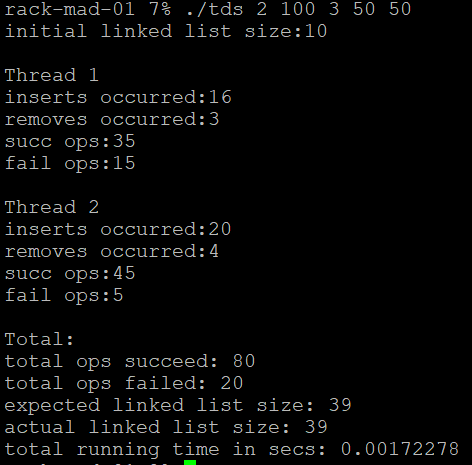
\includegraphics{pasted1}

\subsubsection{Output explenation}

At the beginning we print the initial size of the linked list. After
the workers are done, for each thread we count the amount of inserts
and removes occured, meaning inserts and removes that changed the
data structure state. Also, we count the number of succesful operations
and the number of failure opearations, where here a 'failure' means
that the transaction aborted due to a change in the data structure.
At the end, we print a summary of the details. The output is equal
for all the implementation vesrions.

\subsection{Running all together - the Python script}

To easily run all 4 implementations and compare them, we wrote a python
script named final\_proj\_exp.py (it runs with python version 3.4).
The script gets as an input all the parameters displayed in 5.1.1,
and also the parameters $max\ threads$ and $amount\ runs$. $\forall1\le i\le max\ threads:$
the script runs each implementation with $i$ threads for $amount\ runs$
times, and caclulates the avarage parameters among the $amount\ runs$
runs. In the end, the script creates a plot presenting the differences
among the implementations (the plot is saved under the folder ``out'').

\subsection{Technical details}
\begin{enumerate}
\item All the JAVA code can be found under ``banchmark/src'' in our git
repository. An explenation of how to run the program can be found
in banchmark/README\_COMPILATION.txt.
\item The Python script can also be found under ``banchmark'' directory.
Note: it is important to run the script from within the directory
(so JAVA will be able to access its jarfile). The script arguments
can be seen here:\\
 \includegraphics{\string"python args\string".eps}
\item All the CPP exectuables (tds, tds\_unsafe, tds\_debra) can be found
under ``build''. To compile the CPP program: from within ``build/''
run ``cmake..'', and then: ``make -j''.
\end{enumerate}

\subsection{Code issues:}
\begin{enumerate}
\item When we ran the JAVA implementation from {[}1{]}, we saw that sometimes
the expected size of the linked list at the end of the running doesn't
fit the actual size of the list. The expected size is calculated during
the runtime, by following the amount of inserts and removes operations
that occurred, while the actual linked list size is calculate asynchronously
by iterating the linked list with a counter in the end of the running.
In this project we used the JAVA code as a black box, but maybe it
follows from unsolved edge cases in the index implementation we observed.
\item Sometimes our CPP implementation crushes due to allocating issues.
After trying to understand the problem, we found that, despite the
assumption we based on when we wrote the code, CPP shared\_ptr's are
not thread safe in some edged cases (as described in https://stackoverflow.com/questions/42172988/c11-shared-pointer-thread-safety-is-broken).
But, this bug happens rarely, and after running a bunch of tests we
didn't find uncorrectness issues in our code.
\end{enumerate}

\section{Results and Conclusions}

\subsection{The Results}

The results here present a running example of 10000 tasks, 10 tasks
per transaction, and each measure was taken as the average case of
10 samples. Again, operations are considered as succeed if they were
not aborted by the transaction mechanism (it is a normal behaviour).

\subparagraph{mixed case (50-50 percent of inserts and removes)\protect \\
}

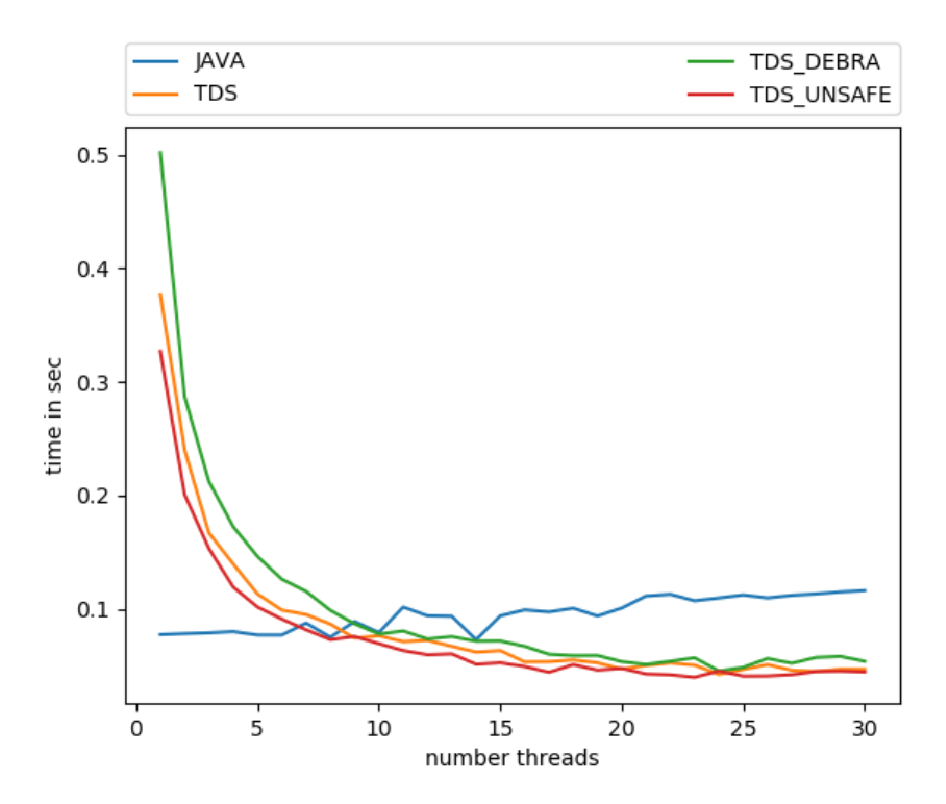
\includegraphics[scale=0.5]{50_50_times}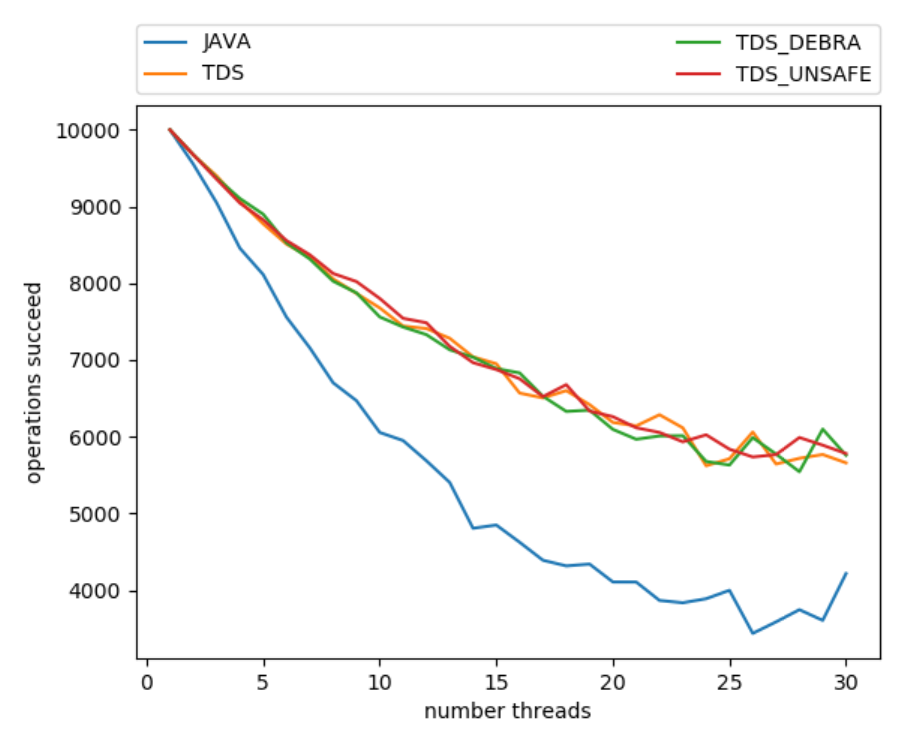
\includegraphics[scale=0.5]{50_50_succ_ops}

\subparagraph{inserts case (all tasks are inserts)\protect \\
}

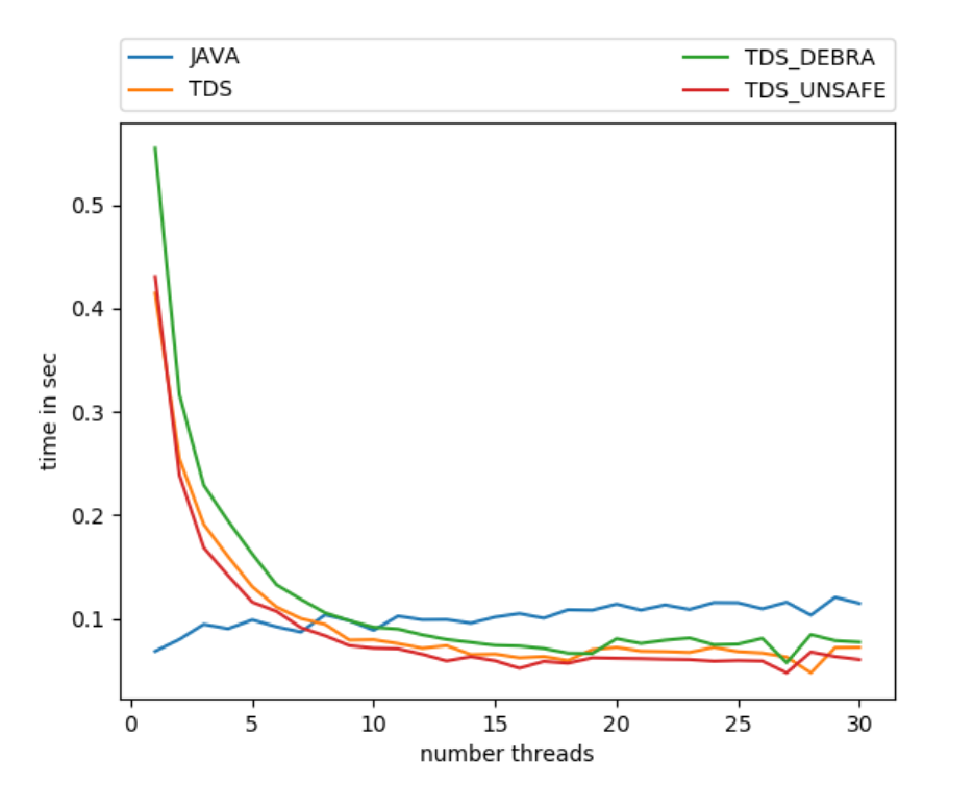
\includegraphics[scale=0.5]{100_inserts_times} 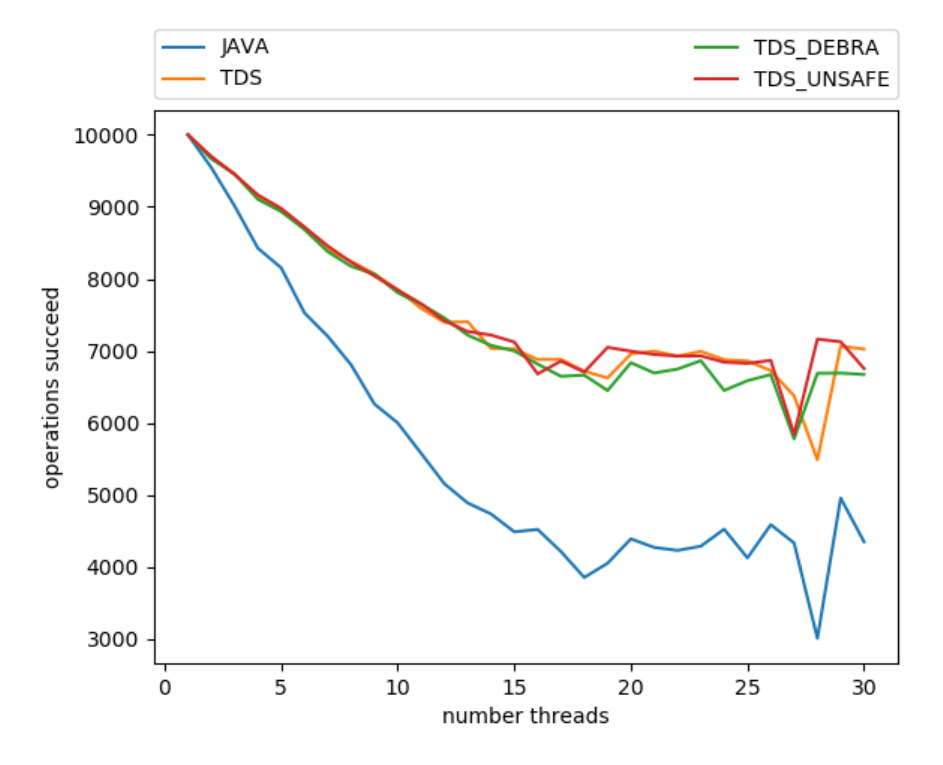
\includegraphics[scale=0.5]{100_inserts_succ_ops}

\subsection{Conclusions}
\begin{enumerate}
\item We can see that there is not a big difference between the mixed case
and the inserts case. This behaviour makes sense, because there is
not a big difference between the two operations in the aspect of the
algorithm.
\item We see that when we run with more threads, more operations fail due
to transaction abort, as we would expect.
\item We can see that in terms of perofrmence, the CPP implementation is
doing better then the JAVA implementation, when running with more
then \textasciitilde{}10 threads. It is important to mention that
we suspected that maybe for some reason the JAVA implementation from
{[}1{]} is not running in parallel. To check this option, we added
print commands inside the workers code and made sure the messages
were printed alternately. For that reason we believe the JAVA implementation
does run in prarllel. Understanding the dieffrences between the implementations
might be tricky, because there are many aspects of differences between
JAVA and CPP. But, since we see that our CPP implementation runs faster
then the JAVA implementation from {[}1{]} only after using a few threads,
and regardless to the caring of memory leak in the CPP code, we assume
this gap is more attached with the general differences between JAVA
and CPP and is not necessarily directly related to the memory cleaning.
\item It seems that there are not dramatic differences between the CPP implementations.
Yet, the experiments above shows that in general, running in unsafe
mode is faster then running in the non leaking mode, probably due
to the clear overhead of ensuring the safetiness of the second. Whats
is maybe more surprising, is that using debra is a bit slower then
using the safe mode. Maybe this fact is related to general overhead
of Debra implementation as it uses more complicated methods.
\end{enumerate}

\section{Future Work}
\begin{enumerate}
\item Add template wrapper for all of our structs (INdexNode, Qnode,…) 
\end{enumerate}
\bibliographystyle{plain}
\bibliography{bibfile}

\end{document}
